\chapter{Functional design} \label{chap:func_design}
\section{Background knowledge}
\subsection{Spin states}
Spin, at least in quantum mechanics, is the intrinsic angular momentum of a particle, which is described by the quantum number of the particle. Importantly, it differs from the angular momentum in classical mechanics, which is extrinsic. Spin characterizes systems of particles, usually electrons, using quantum entanglement. This phenomenon refers to the "entanglement", or spin correlation, of a set of particles.

These foundational concepts make it possible to describe quantum systems using various states. The most simple states, used as descriptors, are the energy states. Ground states refer to the system being in an energy minimum. On the other hand, excited states signify that the system has more energy than at its ground state. Additionally, there can be intermediate states during state transition.

While the aforementioned states describe system energy, they have no bearing on the spin. For the purposes of this project, only two spin states need to be explained. The first one is called singlet state. It occurs when an entangled system has a total spin of 0, caused by the mutual cancellation of spin. For example, for a system of two entangled electrons to be a singlet, the two spins would need to point in opposite directions. The second spin state is called triplet and it has a total spin of 1. Triplets can consist of, for instance, two unpaired electrons with aligned spins that sum up to 1. Singlets and triplets both have major distinguishing features and properties, which is why they can be used for quantum sensing. Aside from the difference in spin, triplets tend to have higher energy levels. They also exhibit attraction to magnetic fields, while singlets cannot be influenced directly by magnetism.

%\subsection{Energy levels and state transitions} and Zero-field splitting
\subsection{Zeeman effect}
Discovered by Pieter Zeeman in 1896, the Zeeman effect is another important phenomenon that enables quantum sensing. If under normal circumstances a light-emitting quantum system only emits one spectral line, then when a magnetic field is applied to it the line will split, thus exhibiting the Zeeman effect. In an \gls{nv} center, this phenomenon causes the $\ket{\pm1}$ energy level to split into $\ket{+1}$ and $\ket{-1}$. 

\subsection{Energy levels}\label{chap:energy_levels}
Figure \ref{fig:energylevels} shows the energy level diagram of an \gls{nv} center.

\begin{figure}[ht]
	\centering
	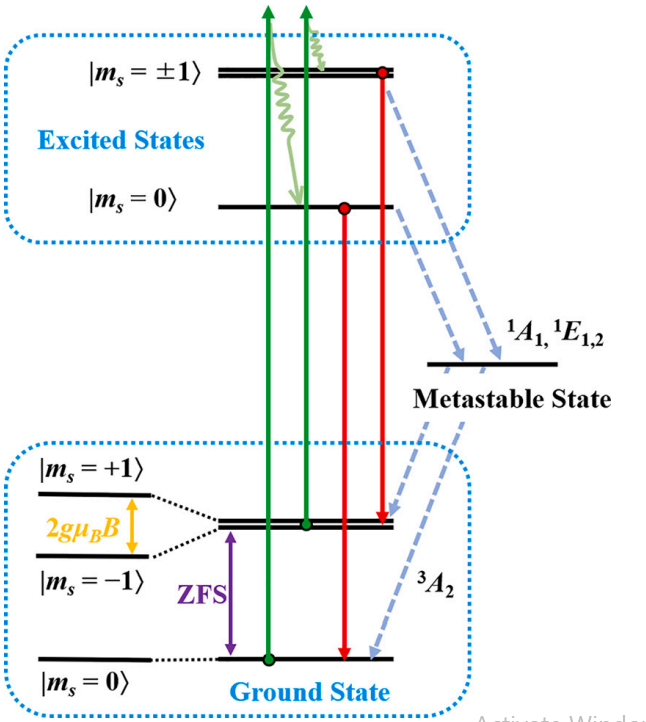
\includegraphics[width=0.7\linewidth]{img/energy_levels}
	\caption{\gls{nv} center energy level diagram (image credit to Song et al \cite{song2024enhancing})}
	\label{fig:energylevels}
\end{figure}

After illuminating the \gls{nv} center with a green laser, electrons go from a ground state to an excited state. They then need to return to the ground state. This decay process is usually direct and emits a red photon, however it can also go through the metastable singlet state and emit an infrared photon. It should be noted that whenever the \gls{nv} center is exposed to the resonant frequency $\nu = 2,87 GHz$ the probability of emitting an infrared photon is significantly increased.


\section{Quantum protocols}
There are a number of different quantum protocols, which differ in what they can measure, in how precisely they can measure it and in the complexity of the hardware they require to operate. \gls{cwodmr} is the main protocol this project is aimed at facilitating. As Saijo et al \cite{saijo2018ac} demonstrate, \gls{cwodmr} is relatively simple, while still detecting magnetic field with reasonable sensitivity. \gls{podmr} does outperform \gls{cwodmr} \cite{zhang2020high}, but because of the added complexity working with it is a "Could have" (see Chapter \ref{project_boundaries}). Before being able to run \gls{podmr} on the setup at the lab, several protocols need to be implemented first \cite{sewani2020coherent}. $T_1$ measurements, which are one of the fundamentals of \gls{mri}, should be conducted first. Afterwards, Rabi oscillations need to be observed and measured in order to calibrate the setup. Without these intermediate protocols, \gls{podmr} cannot be performed.



\subsection{\glsfmtshort{cwodmr}}
\gls{cwodmr} is a quantum protocol that has seen extensive usage in sensing setups that measure magnetic fields. Its working principle is centered around the photoluminescence of \gls{nv} centers and the difference in light emission based on spin states. As already discussed in Chapter \ref{chap:energy_levels}, the \gls{nv} center emits less visible light when at the resonant frequency $\nu$. Additionally, two more dips appear on the spectrum if a magnetic field is applied.Calculating the magnetic field can be done using the formula $h\nu = g_e\mu_BB_{AC}$ \footcite[In the formula, $h$ is the Planck constant, $g_e$ is the g-factor of the electron and $\mu_B$ is the Bohr magneton. Knowing all other variables, $B_{AC}$ can easily be calculated.]{enwiki:1301371272}. Figure \ref{fig:cwodmr} shows an example of what a \gls{cwodmr} spectrum might look like. 

\begin{figure}[ht]
	\centering
	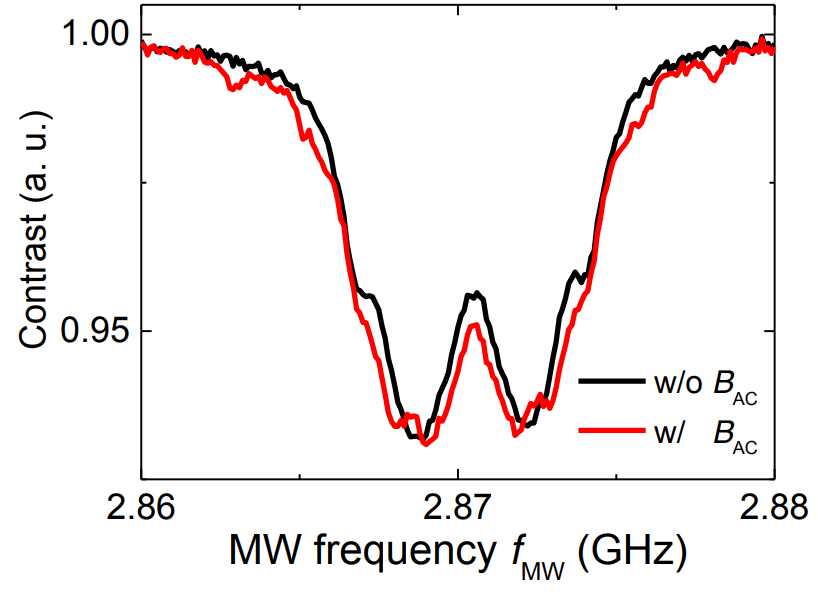
\includegraphics[width=0.7\linewidth]{img/cw_odmr}
	\caption{Example of a \gls{cwodmr} spectrum \textbf{\textcolor{red}{with}} and \textbf{without} a magnetic field (image credit Saijo et al \cite{saijo2018ac})}
	\label{fig:cwodmr}
\end{figure}


\subsection{$T_1$ relaxometry}
$T_1$, $T_2$ and $T_2^*$ relaxation time measurements are commonly associated with radiometry \cite{ballinger23}, but they have other uses too. $T_1$ measurements, in particular, are useful in the realm of quantum sensing. Knowing the $T_1$ relaxation time, which refers to the time it takes for the spins in an \gls{nv} system to decay back to their original state, makes it possible to adjust the pulse sequences of more complex protocols and thus get better results.  %explain what relaxation is and the protcol

% % alternative to tikz diagram
%\begin{figure}[ht]
%	\centering
%	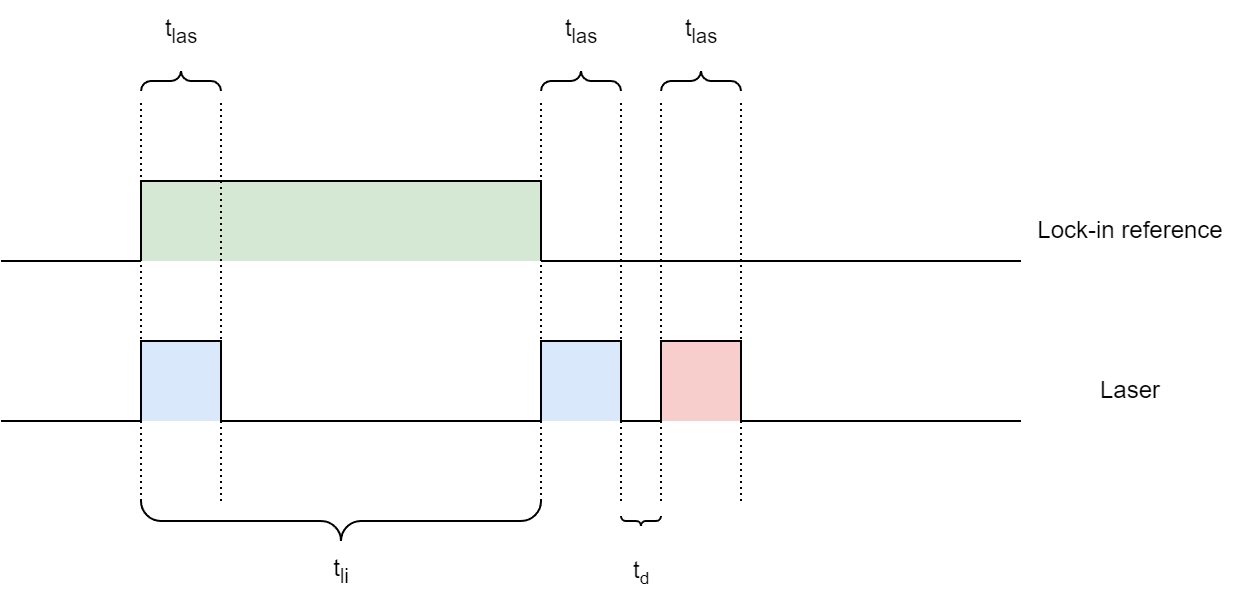
\includegraphics[width=0.9\linewidth]{drawio_diagrams/t1_waveforms.drawio}
%	\caption{Laser and reference signals for $T_1$ measurements}
%	\label{fig:t1waveforms}
%\end{figure}

\begin{figure}[ht]
	\centering
	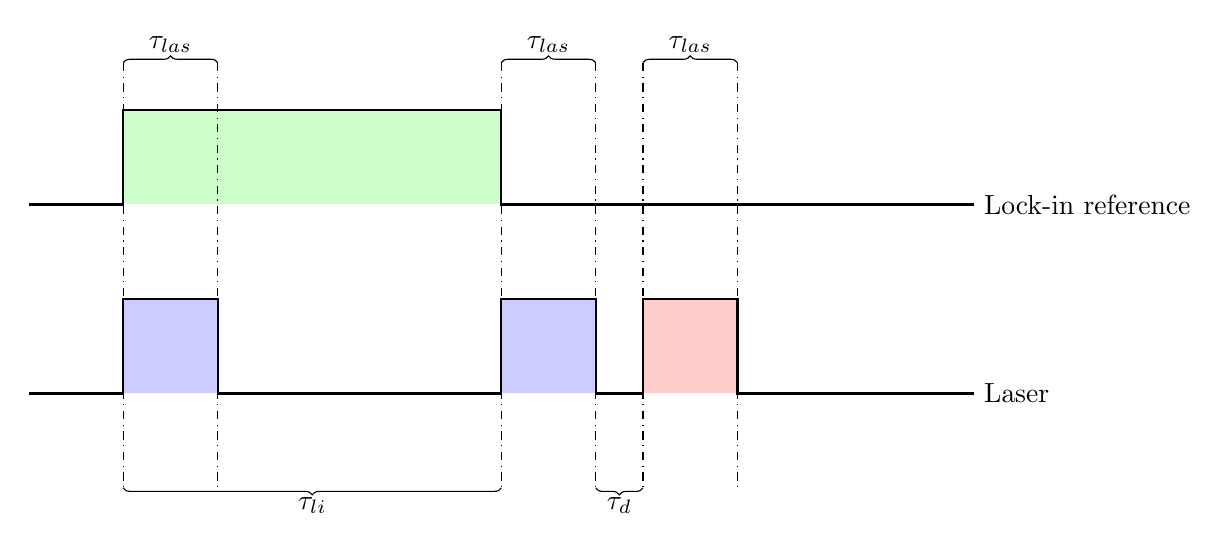
\begin{tikzpicture}[scale=.3]
		% TTL signal rectangles
		\fill [blue!20] 		(4,0) 	rectangle (8,4);
		\fill [blue!20] 		(20,0) 	rectangle (24,4);
		\fill [red!20]			(26,0)	rectangle (30,4);
		\fill [green!20] 		(4,8) 	rectangle (20,12);
		
		% signal lines
		\draw [thick] (0,0) -- (4, 0) -- (4,4) --(8,4) -- (8,0) -- (20,0) -- (20,4) -- (24,4) --(24,0) -- (26,0) -- (26,4) -- (30,4) -- (30,0) -- (40,0) node[anchor=west]{Laser};
		\draw [thick] (0,8) -- (4,8) -- (4,12) -- (20,12) -- (20,8) -- (40,8) node[anchor=west]{Lock-in reference}; % ref
		
		% curly braces top
		\draw [decorate, decoration={brace}] (4,14) -- (8,14) node[midway, above]{$\tau_{las}$};
		\draw [decorate, decoration={brace}] (20,14) -- (24,14) node[midway, above]{$\tau_{las}$};
		\draw [decorate, decoration={brace}] (26,14) -- (30,14) node[midway, above]{$\tau_{las}$};
		
		% curly braces bottom
		\draw [decorate, decoration={brace, mirror}] (4,-4) -- (20,-4) node[midway, below]{$\tau_{li}$};
		\draw [decorate, decoration={brace, mirror}] (24,-4) -- (26,-4) node[midway, below]{$\tau_{d}$};
		
		% dash-dotted lines
		\draw [dash dot] (4,14) -- (4,-4);
		\draw [dash dot] (8,14) -- (8,-4);
		\draw [dash dot] (20,14) -- (20,-4);
		\draw [dash dot] (24,14) -- (24,-4);
		\draw [dash dot] (26,14) -- (26,-4);
		\draw [dash dot] (30,14) -- (30,-4);
		
	\end{tikzpicture}
	\caption{Laser and reference signals for $T_1$ measurements}
	\label{fig:t1waveforms}
\end{figure}





The waveforms which are needed for $T_1$ measurements are shown if Figure \ref{fig:t1waveforms}. While both are important in practice, the lock-in is not as relevant, at least in this section of the report. However, its working principle is explored in Chapter \ref{chap:lockin}. For now, all that needs to be said about the lock-in reference signal is that it is periodic and $\tau_{li}$ is much longer than $\tau_{las}$ (Sewani et al \cite{sewani2020coherent} propose $\tau_{li} = 15 ms$ and $\tau_{las} = 5 \mu s$). Laser pulses, on the other hand, are not periodic. Instead, there are three short pulses every reference period (which is $2\tau_{li} s$ long). The two blue pulses have the same timing every cycle, because they initialize the \gls{nv} spins. However, the red pulse always occurs after the variable dark time $\tau_d$. Depending on the $T_1$ decay at the time of the readout pulse, a different voltage will be detected. Figure \ref{fig:t1result} shows what results can be expected when measuring $T_1$. Determining the value of $T_1$ is done using Formula \ref{eq:t1}, where $I$ is the light intensity, $I_\infty$ is the light intensity offset and $\tau_d$ is the dark time. 

\begin{equation}\label{eq:t1}
I(t)=I_\infty+I(0)e^{-\tau_d/T_1}
\end{equation}



\begin{figure}[ht]
	\centering
	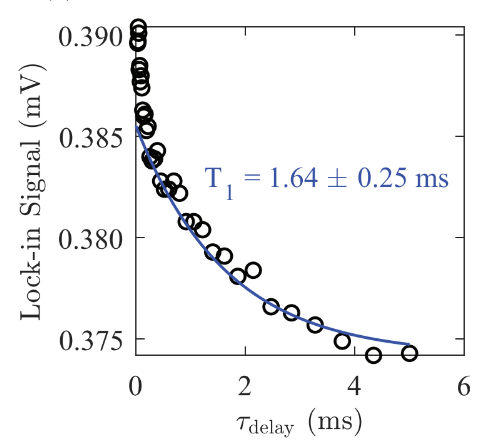
\includegraphics[width=0.7\linewidth]{img/t1_result}
	\caption{Results of a set of $T_1$ measurements with varied dark time $\tau_d$ (image credit to Sewani et al \cite{sewani2020coherent})}
	\label{fig:t1result}
\end{figure}



\subsection{\glsfmtshort{podmr}}
As a descriptor \gls{podmr} is somewhat vague, which is why it has been used for a number of protocols. Different pulse schemes can result in radically different . Some researches use 

\section{Lock-in amplification} \label{chap:lockin}
\section{Quantum sensing setup}
\section{Photodetection \glsfmtshort{pcb}}
Photodetection is how the \gls{nv} photoluminescence is measured, effectively turning light into current using a photodiode. However, a bare photodiode cannot be connected to a lock-in amplifier, because it functions as a current generator. This is where the photodetection \gls {pcb} comes in. Its purpose is to transform the current into voltage and then amplify the resulting signal to the necessary voltage level. 

\subsection{Design process} \label{chap:photodetection_design}
Designing the photodetector is mostly about creating a \gls{tia}, which is a tool used for converting current to voltage, and specifically tuning its parameters so that it works with the selected photodiode under operating conditions. 

\begin{figure}[ht]
	\centering
	\resizebox{.5\textwidth}{!}{%
		\begin{circuitikz}
			\tikzstyle{every node}=[font=\normalsize]
			\draw [ line width=0.5pt](3.75,10.75) to[empty photodiode,l={ \normalsize $D_1$}] (3.75,9);
			\draw [ line width=0.5pt](6.5,10.25) node[op amp,scale=1] (opamp2) {};
			\draw [ line width=0.5pt](opamp2.+) to[short] (5,9.75);
			\draw [ line width=0.5pt] (opamp2.-) to[short] (5,10.75);
			\draw [ line width=0.5pt](7.7,10.25) to[short](8,10.25);
			\draw [line width=0.5pt](5,9) to (5,8.25) node[ground]{};
			\draw [ line width=0.5pt](5,8.5) to[short] (5,9.75);
			\draw [ line width=0.5pt](3.75,10.5) to[short] (3.75,10.75);
			\draw [ line width=0.5pt](3.75,10.75) to[short] (5,10.75);
			\node at (4.5,10.75) [circ] {};
			\draw [ line width=0.5pt](4.5,10.75) to[short] (4.5,13.5);
			\draw [ line width=0.5pt](4.5,12.25) to[short] (5,12.25);
			\draw [ line width=0.5pt](4.5,13.5) to[short] (5,13.5);
			\draw [ line width=0.5pt](7.5,10.25) to[short] (7.5,11);
			\draw [ line width=0.5pt](5,12.25) to[european resistor,l={ \normalsize $R_1$}] (7,12.25);
			\node at (4.5,12.25) [circ] {};
			\draw [ line width=0.5pt](7,12.25) to[short] (7.5,12.25);
			\draw [ line width=0.5pt](7.5,12.25) to[short] (7.5,11);
			\draw [ line width=0.5pt](7.5,12.25) to[short] (7.5,13.5);
			\draw [line width=0.5pt](5,13.5) to[C,l={ \normalsize $C_1$}] (7,13.5);
			\node at (7.5,12.25) [circ] {};
			\draw [ line width=0.5pt](7,13.5) to[short] (7.5,13.5);
			\draw [ line width=0.5pt](8,10.25) to[short, -o] (8.25,10.25) node {$\ \ \ \ \ \ \ \ \ V_{out}$};
			\draw [ line width=0.5pt](3.75,10.75) to[short] (3.75,10.5);
			\draw [line width=0.5pt](3.75,9) to (3.75,8.25) node[ground]{};
			\draw [line width=0.5pt, ->, >=Stealth] (3.25,10.25) -- (3.25,9.25);
			\node [font=\normalsize] at (3,9.75) {$I_f$};
		\end{circuitikz}
	}%
	\caption{Basic \gls{tia} circuit}
	\label{fig:tia}
\end{figure}

The basic circuit, shown in Figure \ref{fig:tia}, is all that is required for photodetection. Following the guidelines for making a \gls{tia} set by Texas Instruments \cite{semig24}, all the parameters of the circuit can be calculated.

\begin{equation}\label{eq:r1}
	R_1 = \frac{V_{o\ max}}{I_{o\ max}}\ \text{assuming}\ V_{o\ min} = 0 \unit{\volt}
\end{equation}

The resistor $R_1$ determines the transimpedance gain of the amplifier. Equation \ref{eq:r1} shows how its value can be calculated by using the output voltage and input current. It should be noted that the minimum output voltage cannot be different from 0 in this use case.

\begin{equation}\label{eq:c1}
	C_1 = \frac{1}{2 \pi R_1 f_{rc}}
\end{equation}

The capacitance of $C_1$ can be calculated using the resistance of $R_1$ and the cutoff frequency $f_{rc}$, as shown in Equation \ref{eq:c1}. 

\begin{equation}\label{eq:gbw}
	f_{c} = (1 + \frac{C_d + C_{cm}}{C_1})f_{rc} \approx f_{rc}
\end{equation}

Even though $f_{rc}$ provides an approximation for the cutoff frequency, the parasitic capacitances in the system will cause it to be slightly bigger. Equation \ref{eq:gbw} shows how a more accurate cutoff frequency $f_c$ can be calculated by taking into account $C_d$ and $C_{cm}$ (differential and common-mode capacitance respectively). In this case, $f_c$ tells us the gain bandwidth or the frequency range in which DC gain is retained.

In addition, a non-inverting amplifier can be added, to increase the gain of the circuit even more, without affecting the phase. Figure \ref{fig:tia_nia} shows how it can be connected to the output of the \gls{tia} from Figure \ref{fig:tia}.

\begin{figure}[!ht]
	\centering
	\resizebox{.9\textwidth}{!}{%
		\begin{circuitikz}
			\tikzstyle{every node}=[font=\normalsize]
			\draw [ line width=0.5pt](3.75,10.75) to[empty photodiode,l={ \normalsize $D_1$}] (3.75,9);
			\draw [ line width=0.5pt](6.5,10.25) node[op amp,scale=1] (opamp2) {};
			\draw [ line width=0.5pt](opamp2.+) to[short] (5,9.75);
			\draw [ line width=0.5pt] (opamp2.-) to[short] (5,10.75);
			\draw [ line width=0.5pt](7.7,10.25) to[short](8,10.25);
			\draw [line width=0.5pt](5,9) to (5,8.25) node[ground]{};
			\draw [ line width=0.5pt](5,8.5) to[short] (5,9.75);
			\draw [ line width=0.5pt](3.75,10.5) to[short] (3.75,10.75);
			\draw [ line width=0.5pt](3.75,10.75) to[short] (5,10.75);
			\node at (4.5,10.75) [circ] {};
			\draw [ line width=0.5pt](4.5,10.75) to[short] (4.5,13.5);
			\draw [ line width=0.5pt](4.5,12.25) to[short] (5,12.25);
			\draw [ line width=0.5pt](4.5,13.5) to[short] (5,13.5);
			\draw [ line width=0.5pt](7.5,10.25) to[short] (7.5,11);
			\draw [ line width=0.5pt](5,12.25) to[european resistor,l={ \normalsize $R_1$}] (7,12.25);
			\node at (4.5,12.25) [circ] {};
			\draw [ line width=0.5pt](7,12.25) to[short] (7.5,12.25);
			\draw [ line width=0.5pt](7.5,12.25) to[short] (7.5,11);
			\draw [ line width=0.5pt](7.5,12.25) to[short] (7.5,13.5);
			\draw [line width=0.5pt](5,13.5) to[C,l={ \normalsize $C_1$}] (7,13.5);
			\node at (7.5,12.25) [circ] {};
			\draw [ line width=0.5pt](7,13.5) to[short] (7.5,13.5);
			\draw [ line width=0.5pt](3.75,10.75) to[short] (3.75,10.5);
			\draw [line width=0.5pt](3.75,9) to (3.75,8.25) node[ground]{};
			\draw [line width=0.5pt, ->, >=Stealth] (3.25,10.25) -- (3.25,9.25);
			\node [font=\normalsize] at (3,9.75) {$I_f$};
			\draw (8,10.25) to[short] (10.25,10.25);
			\draw (11.75,10.75) node[op amp,scale=1] (opamp2) {};
			\draw (opamp2.+) to[short] (10.25,10.25);
			\draw  (opamp2.-) to[short] (10.25,11.25);
			\draw (12.95,10.75) to[short](13.25,10.75);
			\draw (8.5,11.25) to[european resistor,l={ \normalsize $R_2$}] (10.25,11.25);
			\draw (8.5,11.25) to (8.5,11) node[ground]{};
			\draw (11.75,10.75) node[op amp,scale=1] (opamp2) {};
			\draw (opamp2.+) to[short] (10.25,10.25);
			\draw  (opamp2.-) to[short] (10.25,11.25);
			\draw (12.95,10.75) to[short](13.25,10.75);
			\node at (10.25,11.25) [circ] {};
			\draw (10.25,11.25) to[short] (10.25,12.5);
			\draw (10.25,12.5) to[european resistor,l={ \normalsize $R_3$}] (13,12.5);
			\draw (13,12.5) to[short] (13,10.75);
			\draw (13.25,10.75) to[short, -o] (13.5,10.75) node {$\ \ \ \ \ \ \ \ \ V_{out}$};
			\draw (13.5,10.75) to[short, -o] (13.5,10.75) ;
			\node at (7.5,10.25) [circ] {};
			\node [font=\normalsize, anchor=north] at (7.5,10.25) {$V_{ot}$};
			\node [font=\normalsize, anchor=north] at (10.5,11.25) {$V_{-}$};
		\end{circuitikz}
	}%
	\caption{\gls{tia} with non-inverting output amplification}
	\label{fig:tia_nia}
\end{figure}

Equation \ref{eq:nia} is used to calculate the gain of second amplification stage. The formula is derived from the voltage divider formed by the two resistors and the fact that $V_{ot} = V_{-}$.

\begin{equation}\label{eq:nia}
	A_{nia} = \frac{V{out}}{V{ot}} = 1 + \frac{R_3}{R_2}
\end{equation}

The design is based on circuits provided by the client. At their request, the first version of the PCB is an exact replica of the original circuit.  

\section{\glsfmtshort{olia} implementation}
